\subsection{NLP Preprocessing Pipeline} % (fold)
\label{sub:own_pipeline}

\begin{figure}[ht]
  \centering
    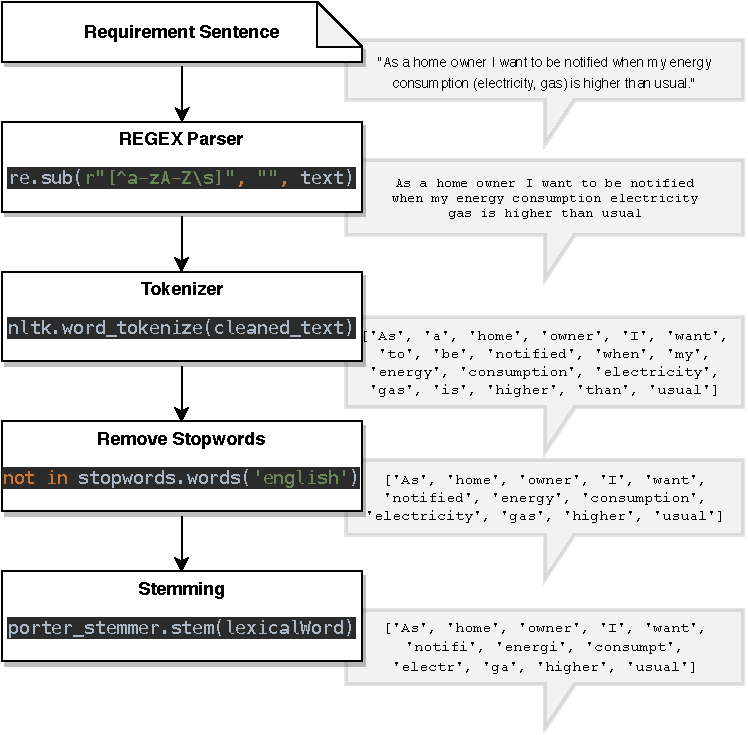
\includegraphics[width=\textwidth]{figures/NLP Pipeline.pdf}
    \caption{Processing an exemplary requirement sentence through our NLP Preprocessing Pipeline.}
    \label{fig:nlp_pipeline}
\end{figure}

As initially described in \autoref{sec:nlp} we preprocessed our requirement documents using an NLP pipeline as shown in \autoref{fig:nlp_pipeline}. Implementing our solution in Python and following the common practice as suggested in \cite{ferrari_natural_2018}, we made use of the NLTK library \cite{nltk_library} to perform the NLP techniques needed for our analysis. As some of the requirements sentences contains special characters, some initial data cleansing was necessary, to remove these special characters (e.g. spaces, dots, apostrophes, slashes) as they would have otherwise been ranked in the later used bag of words. We used regular expressions as provided by the Python standard library in order to do so. For the tokenization, the stop-word-removal and the stemming we used the functions provided by the NLTK API.
% subsection preprocessing (end)